\documentclass[preview]{standalone}
\usepackage{amsmath}
\usepackage{tikz}
\usepackage{mathdots}
\usepackage{yhmath}
\usepackage{cancel}
\usepackage{color}
\usepackage{xcolor}
\usepackage{siunitx}
\usepackage{array}
\usepackage{multirow}
\usepackage{amssymb}
\usepackage{gensymb}
\usepackage{tabularx}
\usepackage{extarrows}
\usepackage{booktabs}
\usetikzlibrary{fadings}
\usetikzlibrary{patterns}
\usetikzlibrary{shadows.blur}
\usetikzlibrary{shapes}
\begin{document}
\begin{center}

\scalebox{0.8}{
  
\tikzset{every picture/.style={line width=0.75pt}} %set default line width to 0.75pt        

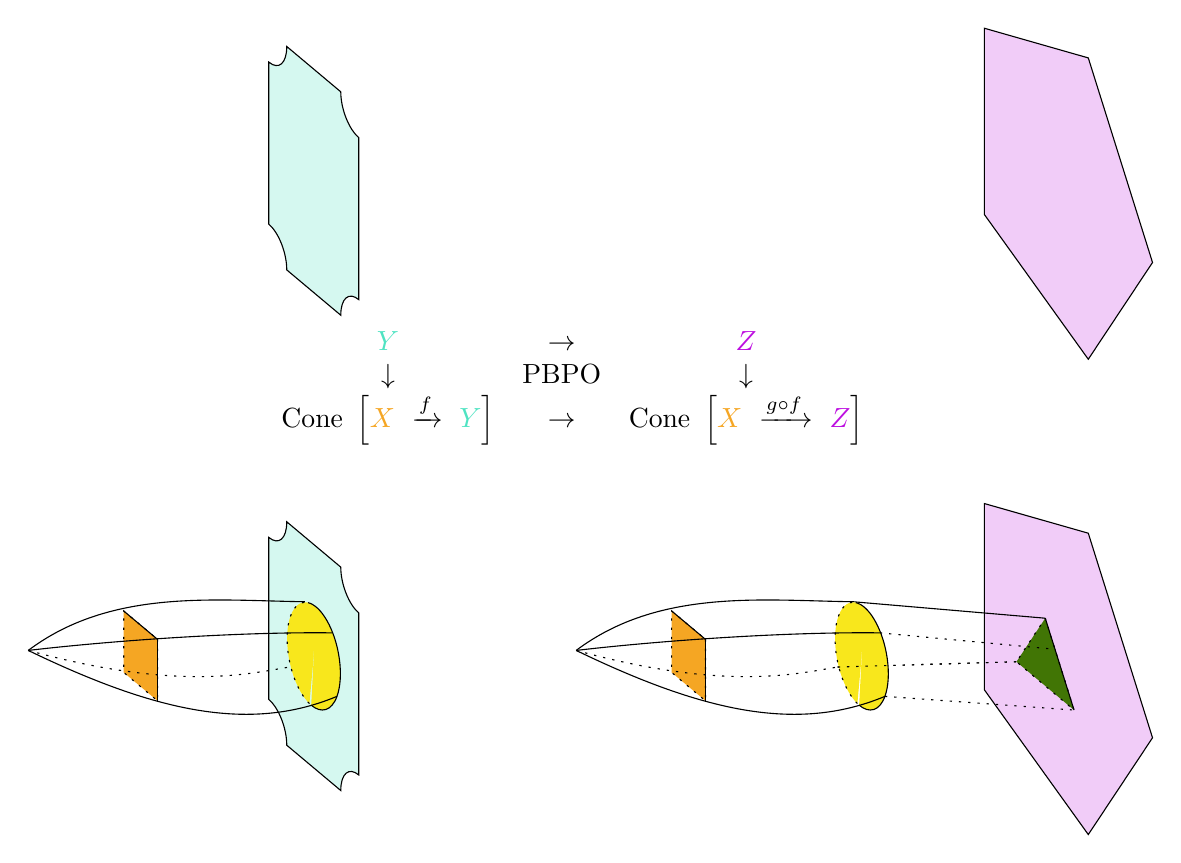
\begin{tikzpicture}[x=0.75pt,y=0.75pt,yscale=-1,xscale=1]
%uncomment if require: \path (0,406); %set diagram left start at 0, and has height of 406

%Shape: Plaque [id:dp8429957223204843] 
\draw  [fill={rgb, 255:red, 80; green, 227; blue, 194 }  ,fill opacity=0.24 ] (164.55,249) .. controls (169.35,253.02) and (173.23,249.66) .. (173.23,241.49) -- (199.25,263.33) .. controls (199.25,271.5) and (203.14,281.37) .. (207.93,285.39) -- (207.93,363.46) .. controls (203.14,359.44) and (199.25,362.8) .. (199.25,370.96) -- (173.23,349.13) .. controls (173.23,340.96) and (169.35,331.09) .. (164.55,327.07) -- cycle ;
%Shape: Arc [id:dp01593962676685856] 
\draw  [draw opacity=0][fill={rgb, 255:red, 248; green, 231; blue, 28 }  ,fill opacity=1 ][dash pattern={on 0.84pt off 2.51pt}] (184.15,329.07) .. controls (182.72,327.68) and (181.3,325.81) .. (179.96,323.49) .. controls (173.78,312.79) and (171.59,296.39) .. (175.06,286.86) .. controls (177.11,281.21) and (180.7,279.24) .. (184.56,280.8) -- (186.24,306.23) -- cycle ; \draw  [dash pattern={on 0.84pt off 2.51pt}] (184.15,329.07) .. controls (182.72,327.68) and (181.3,325.81) .. (179.96,323.49) .. controls (173.78,312.79) and (171.59,296.39) .. (175.06,286.86) .. controls (177.11,281.21) and (180.7,279.24) .. (184.56,280.8) ;  
%Shape: Rectangle [id:dp6634954782215399] 
\draw  [color={rgb, 255:red, 0; green, 0; blue, 0 }  ,draw opacity=1 ][fill={rgb, 255:red, 245; green, 166; blue, 35 }  ,fill opacity=1 ][dash pattern={on 0.84pt off 2.51pt}] (111,298.16) -- (111,327.78) -- (94.67,314.08) -- (94.67,284.46) -- cycle ;
%Curve Lines [id:da6448183100961744] 
\draw    (48.67,303.46) .. controls (88.67,273.46) and (138.67,279.46) .. (182,280) ;
%Curve Lines [id:da46608441863155536] 
\draw  [dash pattern={on 0.84pt off 2.51pt}]  (48.67,303.46) .. controls (121.67,323.46) and (155.67,314.46) .. (174.67,311.46) ;
%Shape: Arc [id:dp9712662896620226] 
\draw  [draw opacity=0][fill={rgb, 255:red, 248; green, 231; blue, 28 }  ,fill opacity=1 ] (183.44,280.44) .. controls (186.42,281.13) and (189.65,283.99) .. (192.52,288.97) .. controls (198.7,299.67) and (200.89,316.07) .. (197.42,325.6) .. controls (194.86,332.65) and (189.9,333.97) .. (185,329.84) -- (186.24,306.23) -- cycle ; \draw   (183.44,280.44) .. controls (186.42,281.13) and (189.65,283.99) .. (192.52,288.97) .. controls (198.7,299.67) and (200.89,316.07) .. (197.42,325.6) .. controls (194.86,332.65) and (189.9,333.97) .. (185,329.84) ;  
%Curve Lines [id:da5133230099250154] 
\draw    (48.67,303.46) .. controls (91.67,298.46) and (151.67,294.46) .. (195,295) ;
%Straight Lines [id:da8179782911340394] 
\draw    (94.67,284.46) -- (111,298.16) ;
%Straight Lines [id:da21362535876354016] 
\draw    (111,298.16) -- (111,327.78) ;
%Curve Lines [id:da34879609878021367] 
\draw    (48.67,303.46) .. controls (108.67,332.46) and (154.67,343.46) .. (197.42,325.6) ;
%Shape: Regular Polygon [id:dp22003839287642313] 
\draw  [fill={rgb, 255:red, 189; green, 16; blue, 224 }  ,fill opacity=0.21 ] (590.35,345.55) -- (559.4,392.17) -- (509.32,322.42) -- (509.32,232.69) -- (559.4,246.99) -- cycle ;
%Shape: Rectangle [id:dp16041223605668264] 
\draw  [color={rgb, 255:red, 0; green, 0; blue, 0 }  ,draw opacity=1 ][fill={rgb, 255:red, 245; green, 166; blue, 35 }  ,fill opacity=1 ][dash pattern={on 0.84pt off 2.51pt}] (375,298.16) -- (375,327.78) -- (358.67,314.08) -- (358.67,284.46) -- cycle ;
%Straight Lines [id:da8911720464956854] 
\draw    (358.67,284.46) -- (375,298.16) ;
%Straight Lines [id:da49428805137506915] 
\draw    (375,298.16) -- (375,327.78) ;
%Straight Lines [id:da41768371326802] 
\draw    (446,280) -- (538.67,287.94) ;
%Shape: Triangle [id:dp8838205291667496] 
\draw  [fill={rgb, 255:red, 65; green, 117; blue, 5 }  ,fill opacity=1 ][dash pattern={on 0.84pt off 2.51pt}] (538.67,287.94) -- (552.54,332.19) -- (524.8,308.92) -- cycle ;
%Straight Lines [id:da5553027421834174] 
\draw  [dash pattern={on 0.84pt off 2.51pt}]  (459,295) -- (543.67,302.94) ;
%Straight Lines [id:da867281520004799] 
\draw  [dash pattern={on 0.84pt off 2.51pt}]  (461.42,325.6) -- (552.54,332.19) ;
%Straight Lines [id:da20266048787719293] 
\draw  [dash pattern={on 0.84pt off 2.51pt}]  (438.67,311.46) -- (524.8,308.92) ;
%Straight Lines [id:da6705537169741107] 
\draw    (552.54,332.19) -- (538.67,287.94) ;
%Curve Lines [id:da6679107186875521] 
\draw    (312.67,303.46) .. controls (352.67,273.46) and (402.67,279.46) .. (446,280) ;
%Curve Lines [id:da8405861660830691] 
\draw  [dash pattern={on 0.84pt off 2.51pt}]  (312.67,303.46) .. controls (385.67,323.46) and (419.67,314.46) .. (438.67,311.46) ;
%Shape: Arc [id:dp24824312434151063] 
\draw  [draw opacity=0][fill={rgb, 255:red, 248; green, 231; blue, 28 }  ,fill opacity=1 ][dash pattern={on 0.84pt off 2.51pt}] (448.15,329.07) .. controls (446.72,327.68) and (445.3,325.81) .. (443.96,323.49) .. controls (437.78,312.79) and (435.59,296.39) .. (439.06,286.86) .. controls (441.11,281.21) and (444.7,279.24) .. (448.56,280.8) -- (450.24,306.23) -- cycle ; \draw  [dash pattern={on 0.84pt off 2.51pt}] (448.15,329.07) .. controls (446.72,327.68) and (445.3,325.81) .. (443.96,323.49) .. controls (437.78,312.79) and (435.59,296.39) .. (439.06,286.86) .. controls (441.11,281.21) and (444.7,279.24) .. (448.56,280.8) ;  
%Shape: Arc [id:dp5160370378999888] 
\draw  [draw opacity=0][fill={rgb, 255:red, 248; green, 231; blue, 28 }  ,fill opacity=1 ] (447.44,280.44) .. controls (450.42,281.13) and (453.65,283.99) .. (456.52,288.97) .. controls (462.7,299.67) and (464.89,316.07) .. (461.42,325.6) .. controls (458.86,332.65) and (453.9,333.97) .. (449,329.84) -- (450.24,306.23) -- cycle ; \draw   (447.44,280.44) .. controls (450.42,281.13) and (453.65,283.99) .. (456.52,288.97) .. controls (462.7,299.67) and (464.89,316.07) .. (461.42,325.6) .. controls (458.86,332.65) and (453.9,333.97) .. (449,329.84) ;  
%Straight Lines [id:da5770180412236376] 
\draw  [dash pattern={on 0.84pt off 2.51pt}]  (438.67,311.46) -- (524.8,308.92) ;
%Curve Lines [id:da715339020149331] 
\draw    (312.67,303.46) .. controls (355.67,298.46) and (415.67,294.46) .. (459,295) ;
%Curve Lines [id:da7764892439898623] 
\draw    (312.67,303.46) .. controls (372.67,332.46) and (418.67,343.46) .. (461.42,325.6) ;
%Shape: Plaque [id:dp5170927333019899] 
\draw  [fill={rgb, 255:red, 80; green, 227; blue, 194 }  ,fill opacity=0.24 ] (164.55,20) .. controls (169.35,24.02) and (173.23,20.66) .. (173.23,12.49) -- (199.25,34.33) .. controls (199.25,42.5) and (203.14,52.37) .. (207.93,56.39) -- (207.93,134.46) .. controls (203.14,130.44) and (199.25,133.8) .. (199.25,141.96) -- (173.23,120.13) .. controls (173.23,111.96) and (169.35,102.09) .. (164.55,98.07) -- cycle ;
%Shape: Regular Polygon [id:dp18597851426162615] 
\draw  [fill={rgb, 255:red, 189; green, 16; blue, 224 }  ,fill opacity=0.21 ] (590.35,116.55) -- (559.4,163.17) -- (509.32,93.42) -- (509.32,3.69) -- (559.4,17.99) -- cycle ;

% Text Node
\draw (169.4,146.57) node [anchor=north west][inner sep=0.75pt]    {$\begin{matrix}
\textcolor[rgb]{0.31,0.89,0.76}{Y} & \rightarrow  & \textcolor[rgb]{0.74,0.06,0.88}{Z}\\
\downarrow  & \text{PBPO} & \downarrow \\
\mathrm{Cone} \ \left[\textcolor[rgb]{0.96,0.65,0.14}{X} \ \xrightarrow{f}\textcolor[rgb]{0.74,0.06,0.88}{\ }\textcolor[rgb]{0.31,0.89,0.76}{Y}\right] & \rightarrow  & \mathrm{Cone} \ \left[\textcolor[rgb]{0.96,0.65,0.14}{X\ }\xrightarrow{g\circ f}\textcolor[rgb]{0.74,0.06,0.88}{\ Z}\right]
\end{matrix}$};


\end{tikzpicture}
}
\end{center}
\end{document}
